\documentclass{beamer}
\usepackage[backend=bibtex,style=numeric,sorting=none]{biblatex}
\usepackage{progressbar}
\usepackage[final]{listings}
\usepackage{graphicx}
\usepackage{wrapfig}
\usepackage{tikz}
\usepackage{tcolorbox}
\usepackage{hyperref}
\usepackage{CJKutf8}
\usepackage{amssymb}
\usepackage{multicol}

\graphicspath{ {./images/} }
\usetheme{AnnArbor}
\addbibresource{main.bib}
\usetikzlibrary{positioning,calc,shapes.multipart}


\title{The Container Security in Healthcare Data Exchange System}
\subtitle{Bachelor's degree graduation project}
\author{Chih-Hsuan Yang}
\institute{National Sun Yat-sen University\\
Advisor: Chun-I Fan
}
\date{\today}

\AtBeginSection[]{
  \begin{frame}
  \vfill
  \centering
  \begin{beamercolorbox}[sep=8pt,center,shadow=true,rounded=true]{title}
    \usebeamerfont{title}\insertsectionhead\par%
  \end{beamercolorbox}
  \vfill
  \end{frame}
}

\begin{document}
\begin{CJK*}{UTF8}{bsmi}

    \begin{frame}
        \titlepage
    \end{frame}

    \begin{frame}{Outline}
        \begin{multicols}{2}
            \tableofcontents
        \end{multicols}
    \end{frame}

    \section{Background}
    \begin{frame}{Backgriund}
        \centering \Huge
        Researching takes time.
    \end{frame}

    \begin{frame}
        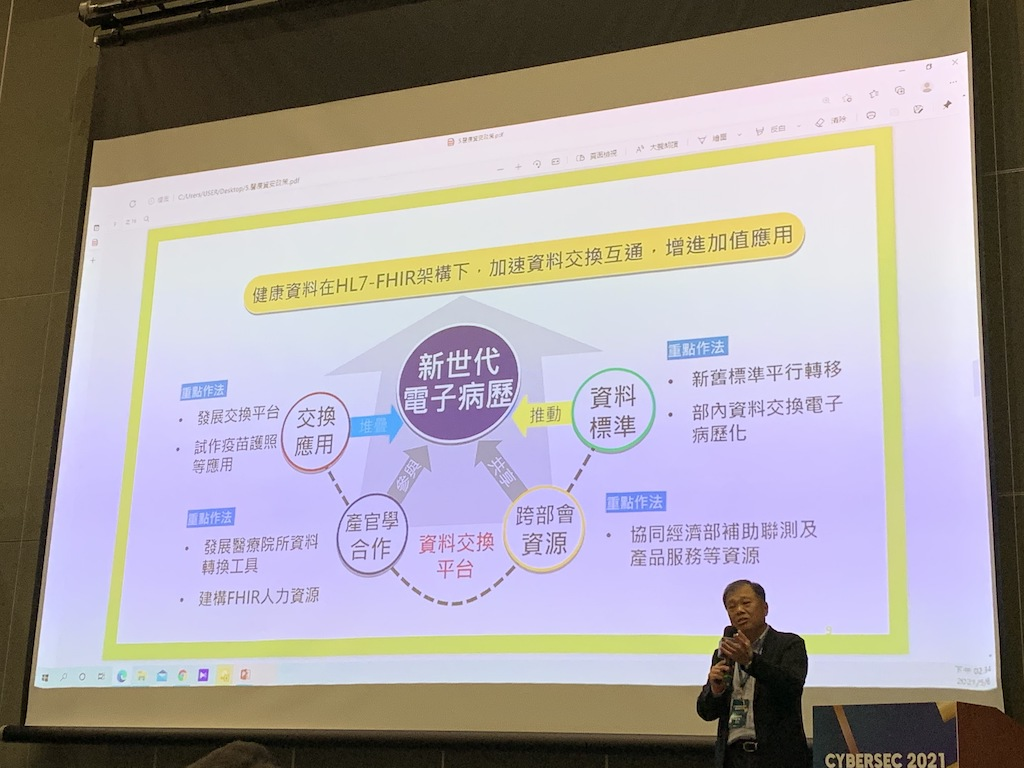
\includegraphics[width=\textwidth]{IMG_6551.jpg}
    \end{frame}

    \begin{frame}
        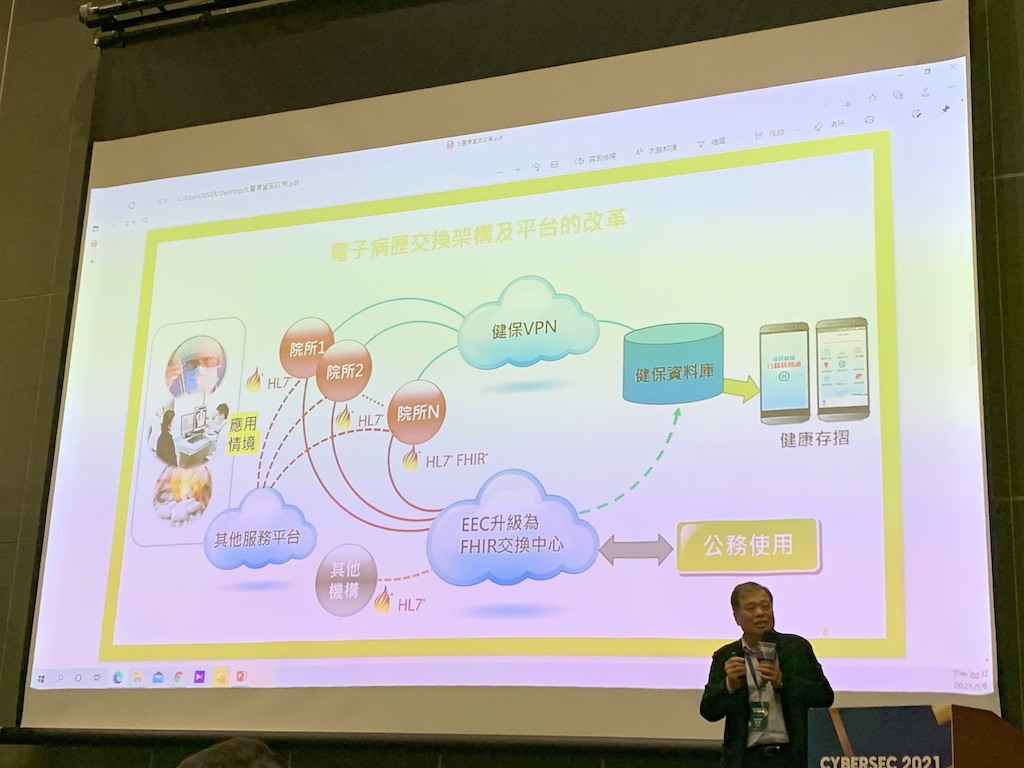
\includegraphics[width=\textwidth]{IMG_6549.jpg}
    \end{frame}

    \section{EEC \& EMR}
    \begin{frame}{2017衛生福利部電子病歷資訊安全檢查表}
        Change password?
        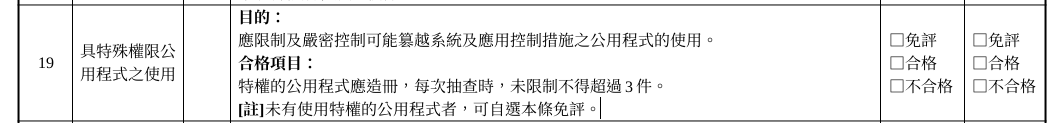
\includegraphics[width=\textwidth]{Screenshot_2021-05-11_15-25-16.png}\\
        Parallel permission
        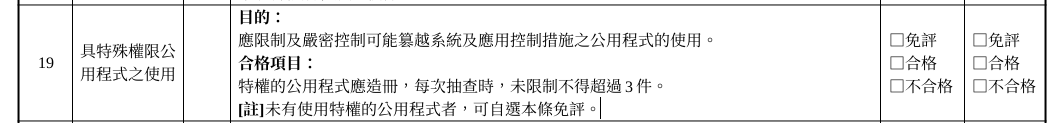
\includegraphics[width=\textwidth]{Screenshot_2021-05-11_15-25-16.png}\\
        Without encryption?
        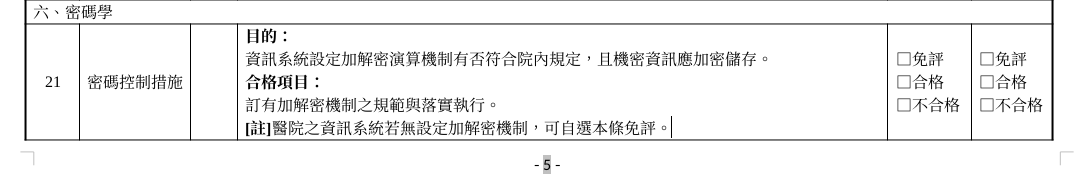
\includegraphics[width=\textwidth]{Screenshot_2021-05-11_15-23-18.png}
    \end{frame}
    \begin{frame}{2017衛生福利部電子病歷資訊安全檢查表}
        FTP? SFTP?
        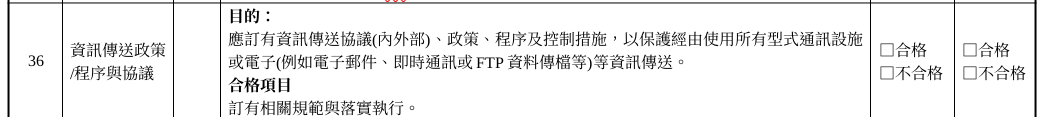
\includegraphics[width=\textwidth]{Screenshot_2021-05-11_15-28-25.png}
        Without certificate?
        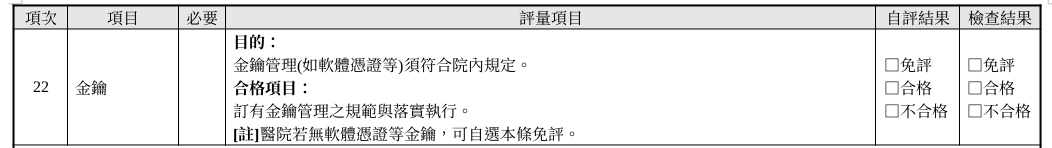
\includegraphics[width=\textwidth]{Screenshot_2021-05-11_15-24-16.png}
    \end{frame}

    \begin{frame}
        \centering
        \Large
        嚴重懷疑沒有經過資安專家審核
    \end{frame}

    \section{Linux source code}
    \begin{frame}
        static \_\_latent\_entropy struct task\_struct *copy\_process
        \begin{itemize}
            \item \href{https://github.com/torvalds/linux/blob/master/kernel/fork.c\#L1851-L2399}{fork.c L1851-2399}
            \item 549
        \end{itemize}

        task\_struct
        \begin{itemize}
            \item \href{https://github.com/torvalds/linux/blob/master/include/linux/sched.h\#L649-L1401}{sched.h L649-1401}
            \item 753
        \end{itemize}
    \end{frame}

    \section{Formal verification}
    \begin{frame}{{Formal verification}}
        \begin{multicols}{2}
            \begin{itemize}
                \setlength\itemsep{1em}
                \item Abstract Interpretation
                \item Formal Model Checking
                \item Theory Prover
            \end{itemize}
            \cite{Software_Engineering_and_Formal_Methods}
            
\includegraphics[height=.8\textheight]{Software_Engineering_and_Formal_Methods.png}
        \end{multicols}

    \end{frame}

    \begin{frame}{Formal verification}
        System architecture for the sample kernel \cite{10.5555/3026877.3026928}
        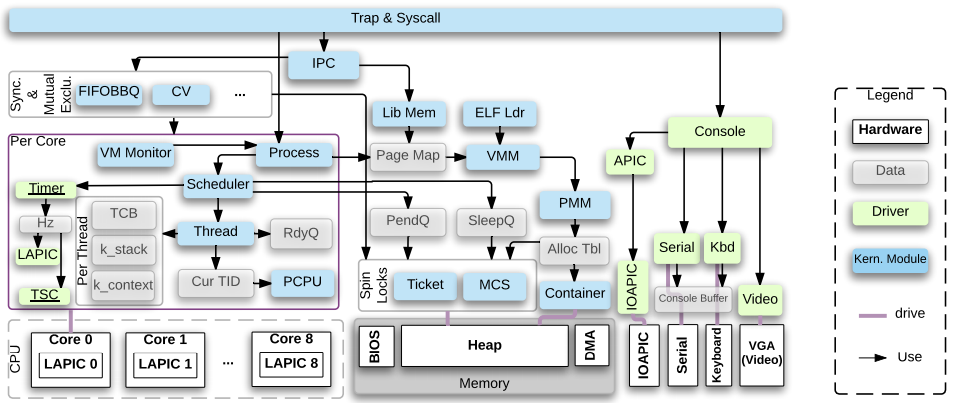
\includegraphics[width=\textwidth]{Screenshot_2021-05-13_15-48-01.png}
    \end{frame}

    \begin{frame}{Formal verification}
        The contextual refinement property about the $s$ kernel can be stated as:
        $$\forall P, [[K \& P]]_{x86mc} \subseteq [[P]]_{s}$$

    \end{frame}

    \begin{frame}{Formal verification}
        $L$: each layer interface \\
        $A$: an active thread set \\
        $EC(L,A)$: set of valid environment contexts\\
        $\prod_{L(A)}(P,\epsilon)$: thread-modular machine\\
        The semantics for a concurrent layer machine L is then:
        $$[[P]]_{L(A)} = \{\prod_{L(A)}(P,\epsilon) \vert \epsilon \in  EC(L,A)\}$$
    \end{frame}

    \begin{frame}{$\lambda$-calculus}
        Formal Small-step Verification of a Call-by-value Lambda Calculus Machine \cite{Kunze_2018}
        \begin{beamerboxesrounded}[shadow=true,width=\textwidth]{Stack}
            $$(T, V ) \gg \sigma := closed(T, V) \wedge (\delta_0@T, \delta_1@V ) = \sigma$$
        \end{beamerboxesrounded}

        \begin{beamerboxesrounded}[shadow=true,width=\textwidth]{Heap}
            $$(T, V, H) \gg (\dot{T}, \dot{V}) \:= T \gg_H \dot{T} \wedge V \gg_H \dot{V}$$

        \end{beamerboxesrounded}
    \end{frame}

    \section{Privacy}
    \begin{frame}{Privacy is not only federated learning}
        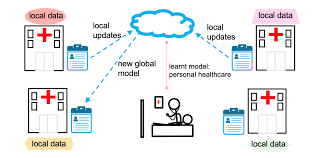
\includegraphics[width=\textwidth]{fl.png}
    \end{frame}

    \begin{frame}{Attribute Based Homomorphic Encryption}
        \def\customHeight{\vrule height 3cm width 0pt}
        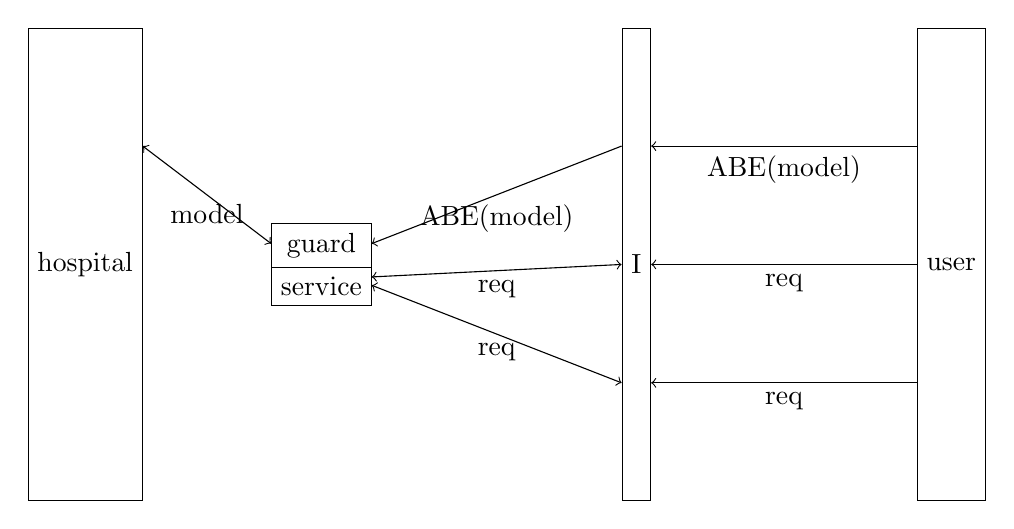
\begin{tikzpicture}
            \node (hospital)[rectangle, draw, minimum height=6cm]{hospital};
            \node (guard)[rectangle split, rectangle split parts=2, draw,
                right of=hospital, xshift=2cm]{\customHeight guard \nodepart{two}\customHeight service};
            \node (I)[rectangle, draw, minimum height=6cm,right of=guard,xshift=3cm]{I};
            \node (user)[rectangle, draw, minimum height=6cm,right of=I,xshift=3cm]{user};
            \draw[<-] ($(I.north east)!0.25!(I.south east)$) -- node[below] {ABE(model)} ($(user.north west)!0.25!(user.south west)$);
            \draw[<-] ($(guard.north east)!0.25!(guard.south east)$) -- node[below] {ABE(model)} ($(I.north west)!0.25!(I.south west)$);
            \draw[<->] ($(hospital.north east)!0.25!(hospital.south east)$) -- node[below] {model} ($(guard.north west)!0.25!(guard.south west)$);
            \draw[<-] ($(I.north east)!0.5!(I.south east)$) -- node[below] {req} ($(user.north west)!0.5!(user.south west)$);
            \draw[<->] ($(guard.north east)!0.65!(guard.south east)$) -- node[below] {req} ($(I.north west)!0.5!(I.south west)$);
            \draw[<-] ($(I.north east)!0.75!(I.south east)$) -- node[below] {req} ($(user.north west)!0.75!(user.south west)$);
            \draw[<->] ($(guard.north east)!0.75!(guard.south east)$) -- node[below] {req} ($(I.north west)!0.75!(I.south west)$);
        \end{tikzpicture}
    \end{frame}

    \section{References}
    \begin{frame}[t, allowframebreaks]
        \frametitle{References}
        \setbeamertemplate{bibliography item}{\insertbiblabel}
        \renewcommand*{\bibfont}{\scriptsize}
        \printbibliography
    \end{frame}

\end{CJK*}
\end{document}